\documentclass[12pt,a4paper]{article}
\newcommand{\LabNumber}{5}
\newcommand{\LabTitle}{Public Key Infrastructure (PKI)\\ și semnături digitale cu OpenSSL}
\newcommand{\LabTitleShort}{Lucrarea de laborator nr. 5 (PKI) — Criptografie \& Securitate Informațională}
% ---------------------------------------------------------------------------
% Common preamble for the CS laboratory reports (compile with XeLaTeX)
% Strunga Daniel-Ioan, FAF-242 — https://github.com/don09dandidi/CS
% ---------------------------------------------------------------------------
\usepackage{fontspec}
\setmainfont{Latin Modern Roman}
\setsansfont{Latin Modern Sans}
\setmonofont{DejaVu Sans Mono}[Scale=0.85]
\usepackage[english]{babel}
\babelprovide[import, main]{romanian}
\usepackage[a4paper, margin=2.5cm, headheight=15pt]{geometry}
\usepackage{amsmath, amssymb}
\usepackage{booktabs, array, longtable, tabularx}
\usepackage{xcolor}
\usepackage{listings}
\usepackage{fvextra}
\usepackage[most]{tcolorbox}
\usepackage{fancyhdr}
\usepackage{tikz}
\usetikzlibrary{arrows.meta, positioning, shapes.geometric, fit, calc}
\usepackage{enumitem}
\usepackage{caption}
\usepackage{float}
\usepackage[hidelinks]{hyperref}
\usepackage{url}

\definecolor{codebg}{RGB}{248,248,250}
\definecolor{codeframe}{RGB}{200,200,210}
\definecolor{kw}{RGB}{0,0,160}
\definecolor{cmt}{RGB}{0,120,0}
\definecolor{str}{RGB}{160,30,30}
\definecolor{termbg}{RGB}{30,32,40}
\definecolor{termfg}{RGB}{225,228,235}
\definecolor{termbar}{RGB}{60,63,75}
\definecolor{boxblue}{RGB}{230,238,250}

\lstdefinestyle{py}{
  language=Python, basicstyle=\ttfamily\small, backgroundcolor=\color{codebg},
  frame=single, rulecolor=\color{codeframe}, numbers=left, numberstyle=\tiny\color{gray},
  keywordstyle=\color{kw}\bfseries, commentstyle=\color{cmt}\itshape, stringstyle=\color{str},
  breaklines=true, showstringspaces=false, columns=fullflexible, keepspaces=true, tabsize=4,
  extendedchars=true, inputencoding=utf8
}
\lstdefinestyle{sh}{
  language=bash, basicstyle=\ttfamily\small, backgroundcolor=\color{codebg},
  frame=single, rulecolor=\color{codeframe}, numbers=left, numberstyle=\tiny\color{gray},
  keywordstyle=\color{kw}\bfseries, commentstyle=\color{cmt}\itshape, stringstyle=\color{str},
  breaklines=true, showstringspaces=false, columns=fullflexible, keepspaces=true
}
\lstdefinestyle{wl}{
  basicstyle=\ttfamily\small, backgroundcolor=\color{codebg},
  frame=single, rulecolor=\color{codeframe}, numbers=left, numberstyle=\tiny\color{gray},
  morekeywords={RandomPrime,RandomInteger,PowerMod,Mod,GCD,FromDigits,IntegerDigits,
    ToCharacterCode,FromCharacterCode,IntegerLength,BitLength,Module,Print,Hash,Length},
  keywordstyle=\color{kw}\bfseries, commentstyle=\color{cmt}\itshape,
  morecomment=[s]{(*}{*)}, breaklines=true, columns=fullflexible, keepspaces=true
}

% Console session box (as in the Lab 2 report)
\newtcolorbox{terminal}[1][Sesiune Terminal Consolă]{
  enhanced, breakable, colback=termbg, colframe=termbar, coltext=termfg,
  fonttitle=\small\ttfamily\bfseries, title={\textbullet\textbullet\textbullet\quad #1},
  left=4pt, right=4pt, top=2pt, bottom=2pt, boxrule=0.6pt, arc=2pt
}
\DefineVerbatimEnvironment{termout}{Verbatim}{fontsize=\scriptsize, breaklines=true, breakanywhere=true}

\newtcolorbox{infobox}[1]{
  enhanced, breakable, colback=boxblue, colframe=kw!60, fonttitle=\bfseries,
  title={#1}, boxrule=0.6pt, arc=2pt
}

\newcommand{\bignum}[1]{\par\nobreak\vspace{1pt}{\noindent\ttfamily\footnotesize\seqsplit{#1}\par}\vspace{5pt}}
\usepackage{seqsplit}

\pagestyle{fancy}
\fancyhf{}
\renewcommand{\headrulewidth}{0.4pt}
\fancyhead[L]{\footnotesize\textit{\LabTitleShort}}
\fancyhead[R]{\footnotesize strunga.daniel-ioan}
\fancyfoot[C]{\thepage}

\newcommand{\makereporttitle}{%
\begin{titlepage}
  \centering
  {\large\bfseries UNIVERSITATEA TEHNICĂ A MOLDOVEI\par}
  \vspace{2pt}
  {\normalsize Facultatea Calculatoare, Informatică și Microelectronică\par}
  {\normalsize Departamentul Ingineria Software și Automatică\par}
  \vspace{5cm}
  {\LARGE\bfseries LUCRAREA DE LABORATOR NR. \LabNumber\par}
  \vspace{8pt}
  {\Large\bfseries \LabTitle\par}
  \vspace{10pt}
  {\normalsize Disciplina: Criptografie și Securitate Informațională\par}
  \vfill
  \begin{tabular*}{\textwidth}{@{}l@{\extracolsep{\fill}}r@{}}
    \textbf{Autor:} & \textbf{Verificat de:} \\
    Daniel-Ioan Strunga & Lector / Supervizor \\
    Student gr. FAF-242 & Maia Zaica \\
  \end{tabular*}
  \vspace{3cm}

  {\normalsize Chișinău — 2026\par}
\end{titlepage}
}


\begin{document}
\makereporttitle
\tableofcontents
\newpage

\section{Introduction and Laboratory Objectives}
Public-key cryptography solves the key distribution problem, but raises a new one: how can a
user be sure that a public key really belongs to the claimed owner? A \textbf{Public Key
Infrastructure} (PKI) answers this question with \textbf{certificates} — public keys bound to an
identity and signed by a trusted \textbf{Certification Authority} (CA). Every participant who
trusts the CA's root certificate can verify any certificate issued by it, and through it any
digital signature produced by the certificate's owner.

Conditions of the laboratory work:
\begin{enumerate}
  \item Create an internal PKI with the \textbf{OpenSSL} tool: generate the root private key and
        initialise a Certification Authority with a \textbf{self-signed certificate}.
  \item The system must be able to \textbf{issue} and \textbf{revoke} keys/certificates for users.
  \item Each user must be able to \textbf{sign} a document/file, and anyone must be able to
        \textbf{verify} the signature.
  \item Requirements: RSA keys; user keys of at least \textbf{2048 bits} with a validity of
        \textbf{365 days}; CA key of \textbf{4096 bits} with a self-signed certificate valid
        \textbf{3650 days} (10 years).
\end{enumerate}
The implementation is a single Bash script, \texttt{lab5\_pki/pki.sh}, which drives the
\texttt{openssl} command-line tool.

\section{Theoretical Foundations}
\subsection{Components of a PKI}
\begin{figure}[H]
\centering
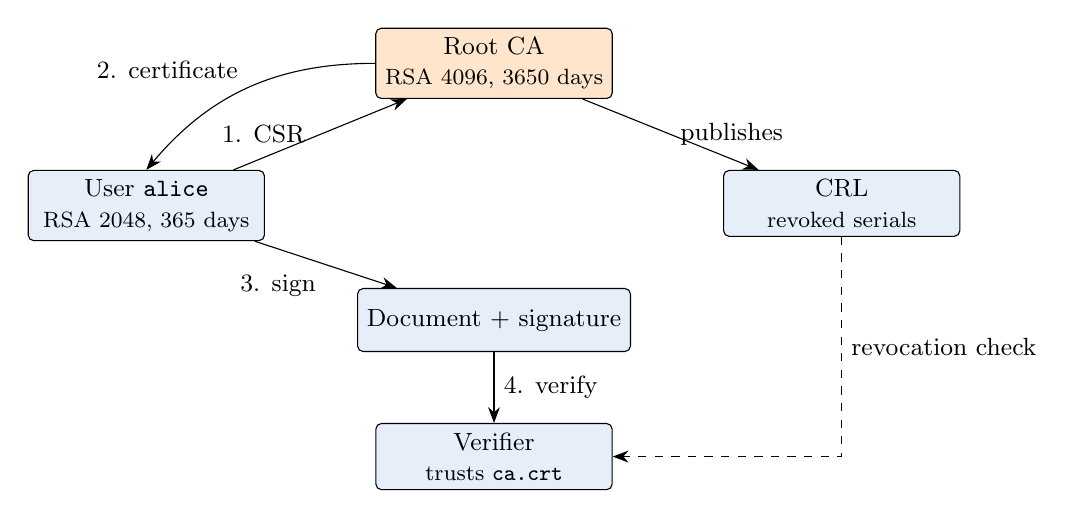
\begin{tikzpicture}[node distance=9mm and 14mm, every node/.style={font=\small},
  box/.style={draw, rounded corners=2pt, minimum width=30mm, minimum height=8mm, fill=boxblue, align=center},
  ar/.style={-{Stealth[length=2mm]}}]
\node[box, fill=orange!20] (ca) {Root CA\\ \footnotesize RSA 4096, 3650 days};
\node[box, below left=of ca] (u1) {User \texttt{alice}\\ \footnotesize RSA 2048, 365 days};
\node[box, below right=of ca] (crl) {CRL\\ \footnotesize revoked serials};
\node[box, below=24mm of ca] (doc) {Document + signature};
\node[box, below=of doc] (v) {Verifier\\ \footnotesize trusts \texttt{ca.crt}};
\draw[ar] (u1) -- node[left, xshift=-2pt]{1. CSR} (ca);
\draw[ar] (ca.west) to[bend right=25] node[above left]{2. certificate} (u1.north);
\draw[ar] (ca) -- node[right]{publishes} (crl);
\draw[ar] (u1) -- node[below left]{3. sign} (doc);
\draw[ar] (doc) -- node[right]{4. verify} (v);
\draw[ar, dashed] (crl) |- node[pos=0.25, right]{revocation check} (v);
\end{tikzpicture}
\caption{Internal PKI implemented in this laboratory}
\end{figure}

\begin{itemize}
  \item \textbf{Certification Authority (CA)} — owns the root key pair; its self-signed X.509
        certificate is the \emph{trust anchor}. The CA keeps a database (\texttt{index.txt}) of all
        issued certificates and their status.
  \item \textbf{Certificate Signing Request (CSR)} — PKCS\#10 structure containing the user's
        public key and identity, signed with the user's private key (proof of possession).
  \item \textbf{X.509 certificate} — subject, issuer, serial number, validity period, public key and
        extensions (\texttt{basicConstraints}, \texttt{keyUsage}), all signed by the CA.
  \item \textbf{Certificate Revocation List (CRL)} — list of serial numbers of revoked
        certificates, signed by the CA; a certificate that is on the CRL must not be trusted even
        before its expiry date (e.g.\ when the private key is compromised).
\end{itemize}

\subsection{RSA Digital Signature}
For a document $M$, a hash function $H$ (SHA-256) and the signer's RSA key pair $(e,n)$, $(d,n)$:
\begin{align}
  \text{signing:}\quad & s = \mathrm{PKCS1\_v1.5}(H(M))^{\,d} \bmod n,\\
  \text{verification:}\quad & s^{e} \bmod n \stackrel{?}{=} \mathrm{PKCS1\_v1.5}(H(M)).
\end{align}
A valid signature guarantees \textbf{integrity} (any change to $M$ changes $H(M)$),
\textbf{authenticity} and \textbf{non-repudiation} (only the owner of $d$ could produce $s$).
The PKI adds the binding between $(e,n)$ and a real identity.

\subsection{Verification Procedure}
A signature is accepted only if \emph{both} checks succeed:
\begin{enumerate}
  \item \textbf{certificate check} — the signer's certificate chains to the trusted CA, is within
        its validity period and is \emph{not} listed in the current CRL;
  \item \textbf{cryptographic check} — the signature verifies with the public key extracted from
        that certificate.
\end{enumerate}

\section{Implementation}
\subsection{Structure of the PKI}
\begin{lstlisting}[style=sh, numbers=none, caption={Files created by \texttt{pki.sh}}]
pki/
|-- ca/
|   |-- openssl.cnf          # CA configuration (policies, extensions)
|   |-- private/ca.key       # root private key, RSA 4096 (chmod 600)
|   |-- certs/ca.crt         # self-signed root certificate, 3650 days
|   |-- crl/ca.crl.pem       # certificate revocation list
|   |-- index.txt, serial, crlnumber, newcerts/   # CA database
`-- users/<user>/
    |-- <user>.key           # user private key, RSA 2048 (chmod 600)
    |-- <user>.csr           # certificate signing request
    |-- <user>.crt           # certificate issued by the CA, 365 days
    `-- <user>.pub.pem       # public key extracted from the certificate
\end{lstlisting}

\subsection{Commands}
\begin{table}[H]
\centering
\caption{Interface of the \texttt{pki.sh} tool}
\begin{tabularx}{\textwidth}{>{\ttfamily}l X}
\toprule
\textrm{Command} & Action \\
\midrule
init-ca & generates the 4096-bit CA key and the self-signed certificate (3650 days), initialises the database and an empty CRL \\
issue <user> & generates a 2048-bit RSA key and a CSR; the CA signs it into a certificate valid 365 days (\texttt{keyUsage = digitalSignature, nonRepudiation}) \\
sign <user> <file> & checks that the user's certificate is still trusted, then signs the file with RSA/SHA-256 \\
verify <user> <file> [sig] & checks the certificate (chain + CRL) and the signature \\
revoke <user> [reason] & revokes the certificate in the CA database and publishes a new CRL \\
list, info <user> & show the CA database / the details of a certificate \\
demo & runs the complete scenario in a temporary directory \\
\bottomrule
\end{tabularx}
\end{table}

\subsection{Key OpenSSL Operations}
\begin{lstlisting}[style=sh, caption={CA initialisation}]
openssl genrsa -out ca/private/ca.key 4096
openssl req -config ca/openssl.cnf -new -x509 -days 3650 -sha256 \
    -key ca/private/ca.key -extensions v3_ca \
    -subj "/C=MD/ST=Chisinau/L=Chisinau/O=UTM FCIM/OU=FAF-242/CN=FAF-242 Root CA" \
    -out ca/certs/ca.crt
openssl ca -config ca/openssl.cnf -gencrl -out ca/crl/ca.crl.pem
\end{lstlisting}

\begin{lstlisting}[style=sh, caption={Issuing a user key and certificate}]
openssl genrsa -out users/alice/alice.key 2048
openssl req -config ca/openssl.cnf -new -key users/alice/alice.key -sha256 \
    -subj "/C=MD/L=Chisinau/O=UTM FCIM/OU=FAF-242/CN=alice" -out users/alice/alice.csr
openssl ca -config ca/openssl.cnf -batch -notext -extensions usr_sign -days 365 \
    -in users/alice/alice.csr -out users/alice/alice.crt
\end{lstlisting}

\begin{lstlisting}[style=sh, caption={Signing, verification and revocation}]
# sign
openssl dgst -sha256 -sign users/alice/alice.key -out doc.txt.alice.sig doc.txt
# verify: 1) certificate (chain + CRL)   2) signature
openssl verify -crl_check -CAfile ca/certs/ca.crt -CRLfile ca/crl/ca.crl.pem users/alice/alice.crt
openssl x509 -in users/alice/alice.crt -pubkey -noout > alice.pub.pem
openssl dgst -sha256 -verify alice.pub.pem -signature doc.txt.alice.sig doc.txt
# revoke + publish new CRL
openssl ca -config ca/openssl.cnf -revoke users/alice/alice.crt -crl_reason keyCompromise
openssl ca -config ca/openssl.cnf -gencrl -out ca/crl/ca.crl.pem
\end{lstlisting}

The CA configuration defines the extensions of the issued certificates:
\begin{lstlisting}[style=sh, numbers=none, caption={Certificate extensions (\texttt{openssl.cnf})}]
[ v3_ca ]
basicConstraints = critical, CA:true
keyUsage         = critical, digitalSignature, cRLSign, keyCertSign
[ usr_sign ]
basicConstraints = critical, CA:false
keyUsage         = critical, digitalSignature, nonRepudiation
extendedKeyUsage = codeSigning, emailProtection
\end{lstlisting}

\section{Results — Complete Scenario}
The command \texttt{./pki.sh demo} executes the full life cycle. The relevant parts of the output
are shown below.

\subsection{CA Initialisation and Certificate Issuing}
\begin{terminal}
\begin{termout}
========== 1. Initialise the CA ==========
[*] Generating the CA root private key (RSA 4096 bits)
[*] Creating the self-signed CA certificate (valid 3650 days)
[OK] CA initialised
subject=C = MD, ST = Chisinau, L = Chisinau, O = UTM FCIM, OU = FAF-242, CN = FAF-242 Root CA
issuer=C = MD, ST = Chisinau, L = Chisinau, O = UTM FCIM, OU = FAF-242, CN = FAF-242 Root CA
notBefore=Nov 15 11:31:22 2026 GMT
notAfter=Nov 12 11:31:22 2036 GMT

========== 2. Issue keys for alice and bob ==========
[*] Generating private key for 'alice' (RSA 2048 bits)
[*] Creating the certificate signing request (CSR)
[*] CA signs the CSR -> certificate valid 365 days
[OK] Issued certificate for 'alice'
subject=C = MD, L = Chisinau, O = UTM FCIM, OU = FAF-242, CN = alice
issuer=C = MD, ST = Chisinau, L = Chisinau, O = UTM FCIM, OU = FAF-242, CN = FAF-242 Root CA
notBefore=Nov 15 11:31:22 2026 GMT
notAfter=Nov 15 11:31:22 2027 GMT
serial=1000
\end{termout}
\end{terminal}
The CA certificate is self-signed (subject = issuer) and valid 10 years; the user certificate is
issued by the CA and valid exactly 365 days.

\subsection{Signing and Verification}
\begin{terminal}
\begin{termout}
========== 3. alice signs a document ==========
[OK] 'alice' signed /tmp/demo/contract.txt -> /tmp/demo/contract.txt.alice.sig (256 bytes, RSA/sha256)
     sha256(file) = cd354cf4afaf7df53aceade63a6bdbb12ed55ca6e41b898799676cc2a5fbf92e

========== 4. Verification ==========
[*] 1) Certificate chain + revocation check (CA + CRL)
/tmp/demo/pki/users/alice/alice.crt: OK
[OK] certificate of 'alice' is valid and not revoked
[*] 2) Cryptographic signature check with the public key from the certificate
Verified OK
[OK] RESULT: signature of 'alice' on /tmp/demo/contract.txt is VALID
\end{termout}
\end{terminal}
The signature has 256 bytes = 2048 bits, the size of the signer's modulus.

\subsection{Negative Tests: Modified Document and Wrong Signer}
\begin{terminal}
\begin{termout}
========== 5. Tampered document ==========
[OK] certificate of 'alice' is valid and not revoked
... rsa routines:ossl_rsa_verify:bad signature
Verification failure
[FAIL] RESULT: signature of 'alice' on /tmp/demo/contract_modified.txt is REJECTED

========== 6. Wrong signer (bob's certificate) ==========
[OK] certificate of 'bob' is valid and not revoked
... rsa routines:RSA_padding_check_PKCS1_type_1:invalid padding
Verification failure
[FAIL] RESULT: signature of 'bob' on /tmp/demo/contract.txt is REJECTED
\end{termout}
\end{terminal}
Adding one line to the document changes its SHA-256 digest, so the signature no longer matches
(integrity). Verifying Alice's signature with Bob's public key fails at the PKCS\#1 padding check
(authenticity).

\subsection{Revocation}
\begin{terminal}
\begin{termout}
========== 7. Revoke alice ==========
[*] Revoking certificate of 'alice' (reason: keyCompromise)
[OK] Certificate revoked, CRL updated: /tmp/demo/pki/ca/crl/ca.crl.pem
    Serial Number: 1000
        Revocation Date: Nov 15 11:31:23 2026 GMT
                Key Compromise

========== 8. Verification after revocation ==========
[*] 1) Certificate chain + revocation check (CA + CRL)
C = MD, L = Chisinau, O = UTM FCIM, OU = FAF-242, CN = alice
error 23 at 0 depth lookup: certificate revoked
[FAIL] certificate of 'alice' is NOT trusted (revoked or invalid)
[*] 2) Cryptographic signature check with the public key from the certificate
Verified OK
[FAIL] RESULT: signature of 'alice' on /tmp/demo/contract.txt is REJECTED

========== 9. Revoked user tries to sign ==========
[FAIL] certificate of 'alice' is revoked or invalid — signing refused

========== 10. CA database ==========
STATUS EXPIRES          SERIAL   SUBJECT
REVOKED 271115113122Z    1000     /C=MD/L=Chisinau/O=UTM FCIM/OU=FAF-242/CN=alice
valid  271115113123Z    1001     /C=MD/L=Chisinau/O=UTM FCIM/OU=FAF-242/CN=bob
\end{termout}
\end{terminal}
After revocation the signature is still mathematically correct (\texttt{Verified OK}), but it is
rejected because the certificate appears in the CRL — exactly the purpose of revocation when a
private key is compromised. The tool also refuses to produce new signatures with a revoked key.
A new key and certificate can then be issued for the same user (\texttt{./pki.sh issue alice}).

\section{Source Code and Repository}
\begin{center}
\url{https://github.com/don09dandidi/CS} \quad (directory \texttt{lab5\_pki/})
\end{center}
\subsection{Build and Execution Instructions}
\begin{lstlisting}[style=sh]
git clone https://github.com/don09dandidi/CS.git
cd CS/lab5_pki
chmod +x pki.sh
./pki.sh demo                       # full scenario in a temporary directory
# or step by step:
./pki.sh init-ca
./pki.sh issue daniel
./pki.sh sign daniel raport.pdf
./pki.sh verify daniel raport.pdf
./pki.sh revoke daniel keyCompromise
./pki.sh list
\end{lstlisting}
The script works with OpenSSL 1.1/3.x and with the LibreSSL build shipped with macOS. The
\texttt{pki/} directory (which contains private keys) is excluded from Git via \texttt{.gitignore}.

\section{Conclusion}
\begin{enumerate}
  \item An internal PKI was built with OpenSSL: a root CA with a 4096-bit RSA key and a
        self-signed certificate valid 3650 days, issuing 2048-bit RSA user certificates valid 365
        days, as required.
  \item The full certificate life cycle was implemented — key generation, CSR, issuing,
        revocation with a reason code, and CRL publication.
  \item Users sign files with RSA/SHA-256; verification combines the certificate check (chain of
        trust and CRL) with the cryptographic check of the signature.
  \item The negative tests confirmed the three properties of digital signatures: a modified
        document, a wrong signer and a revoked certificate are all rejected.
\end{enumerate}

\begin{thebibliography}{9}
\bibitem{x509} D.\ Cooper et al., \emph{RFC 5280: Internet X.509 Public Key Infrastructure
  Certificate and CRL Profile}, 2008.
\bibitem{pkcs1} K.\ Moriarty et al., \emph{RFC 8017: PKCS \#1: RSA Cryptography Specifications
  Version 2.2}, 2016.
\bibitem{openssl} OpenSSL Project, \emph{openssl-ca(1), openssl-req(1), openssl-dgst(1) manual pages}.
\bibitem{medium} Y.\ Bilgiç, \emph{Create self-signed certificates and keys with OpenSSL}, Medium.
\bibitem{stallings} William Stallings, \emph{Cryptography and Network Security: Principles and
  Practice}, 7th Edition, Pearson, 2017.
\end{thebibliography}
\end{document}
